
\section{Xapian}

\subsection{Installation}

Der empfohlene Installationsweg für Xapian führt über das Paketquelle (PPA) der Entwickler. Nachdem dieses eingefügt wurde, kann Xapian entweder in einer C++ oder Python Variante installiert werden. Damit Xapian auch mit PHP anzusprechen ist, ist es allerdings notwendig den PHP-Connector aus Lizenzgründen selbst zu bauen. Dabei muss vorher der ein Eintrag, der ausweist, dass aus dieser Quelle auch Source-Code geladen werden kann, in der Paketquellen hinzugefügt werden. Nachdem nun der PHP-Klient gebaut worden ist, kann dieser nun normal installiert werden.
Allerdings ist der Server bisher nur Lokal ansprechbar, um dies zu ändern, muss ein TCP-Server für Xapian gestartet werden. Um diesen zu Nutzen ist es vonnöten ein weiteres Paket aus der PPA zu installieren. Damit nun der Server gestartet werden kann, muss zuerst ein Index, der bei Xapian Database genannt wird, gebaut werden. Dazu mehr in dem Teil \ref{xap:index}. Danach kann der Server auf einen beliebigen Port gestartet werden.

\subsection{Indexierung}
\label{xap:index}

Durch die fehlende Dokumentation zur Indexierung von MySQL-Datenbanken, habe ich zuerst einmal das gegebene Beispiel zur Indexierung von einer CSV Datei durchgearbeitet. Dabei ist mir aufgefallen, dass hier die Indexierung komplett selbst geschrieben werden muss. Deswegen habe ich anhand des Beispiels eine Indexierung für die MySQL-Daten geschrieben. 

\begin{lstlisting}[language=php, frame=single, label={lst:managedSchema}, 
	morekeywords={type,uninvertible,indexed,stored,field,multiValued, name}] 
	<?php
	require_once("xapian.php");
	
	//Open MYSQL-Connection and Run Query. Save the Output in $result
	
	// Create or open the database we're going to be writing to.
	$db = new XapianWritableDatabase($xapianDb, Xapian::DB_CREATE_OR_OPEN);
	// Set up a TermGenerator that we'll use in indexing.
	$termgenerator = new XapianTermGenerator();
	$termgenerator->set_stemmer(new XapianStem('de')); //Setup Stemmer
	
	while ($row = $result->fetch_assoc()) { //Loop through MySQL-Rows
	
		$identifier = $row['id'];
		unset($row['id']);
		// Create new Row for the starting Letter
		$searchIndexLetter = $row['original_bezeichnung'][0];

		$doc = new XapianDocument(); // Create new Document
		$termgenerator->set_document($doc); //Put it into the Term-Generator
	
		// Index the field with a suitable prefix.
		$termgenerator->index_text($searchIndexLetter, 1, 'K'); 
		// Make it available for Search
		$termgenerator->index_text($searchIndexLetter); 
	
		foreach ($row as $index) {
			if ($index = '') { //Xapian cant Index Empty Fields
				$index = 'EMPTY';
			}
			$termgenerator->increase_termpos(); // Make Space between Entries
			$termgenerator->index_text($index); // Add Every Field
		}
		$doc->set_data(json_encode($row)); // Store all the fields
	
		$idterm = "Q".$identifier; //Set ID to not have Duplicates
		$doc->add_boolean_term($idterm);
		$db->replace_document($idterm, $doc);
	}
	$conn->close();
	
  \end{lstlisting}

Bei dem Skript möchte ich gerne auf ein paar Zeilen genauer eingehen. Zuerst in Zeile 10. Der Stemmer dient dazu, wenn der Plural eines Wortes gesucht wird, auch Ergebnisse mit dem Singular zu finden. In Zeile 23 wird ein Feld mit einem Präfix indexiert, dies dient dazu diese Zeile für die spätere Suche auszuweisen. Die Präfixe werden dabei vor die Zeile geschrieben und bei der Suche dann wieder herausgefiltert. Die anderen Felder wurde für die generelle Suche ohne Präfix indexiert. Damit ein Feld allerdings indexiert werden kann, darf es nicht leer sein. Deswegen habe ich leere Felder mit EMPTY gekennzeichnet. 

Als nun das PHP-Script auf den Server gestartet wurde, mussten noch eine Warnung behoben werden. Dazu wurde die php.ini angepasst, indem der Eintrag 'enable\_dl' aktiviert wurde. 

Die Indexierung lief dabei äußerst schnell in unter einer Minute ab.

\subsection{Oberfläche}

Xapian besitzt keine Oberfläche zur Verwaltung. Allerdings kann sich ein Such-Frontend installiert werden, welches allerdings hier nicht geprüft wurde, da die Dokumentation noch nicht verfügbar war. Generell würde das Projekt ein selbstgebautes Frontend benötigen.

\subsection{Dokumentation}

Bei dem letzten Versionsupgrade wurde die Dokumentation von Xapian komplett umgeschrieben. Diese neue Dokumentation hat bisher noch viele Lücken und besitzt auch Todo-Boxen \ref{img:xapianDoku}.
Zu der Installation von dem TCP-Server war nichts in der neuen Dokumentation zu finden. Beim Durchsuchen des Internets, wie der Server extern ansprechbar gemacht werden kann, bin ich zufällig auf eine Seite der alten Dokumentation gestoßen, welche einen Befehl zum Starten vermerkt hatte. Nachdem dieser Befehl ausgeführt wurde, wurde gemeldet, dass für diesen Befehl ein weiteres Paket installiert werden musste. Dieses Paket wurde in der Dokumentation nicht vermerkt. 

Generell bietet die Dokumentation bisher nur einen sehr grundlegenden Einblick in das System und beleuchtet keine genauen Themen, wie das Indexieren von MySQL-Datenbanken. Positiv anzumerken ist allerdings, dass Xapian ein Beispiel zu Indexierung von Daten mit Code in allen verfügbaren Sprachen bereitstellt. In der Dokumentation direkt ist allerdings nur das Python-Beispiel erklärt.

\begin{figure}
	\centering
	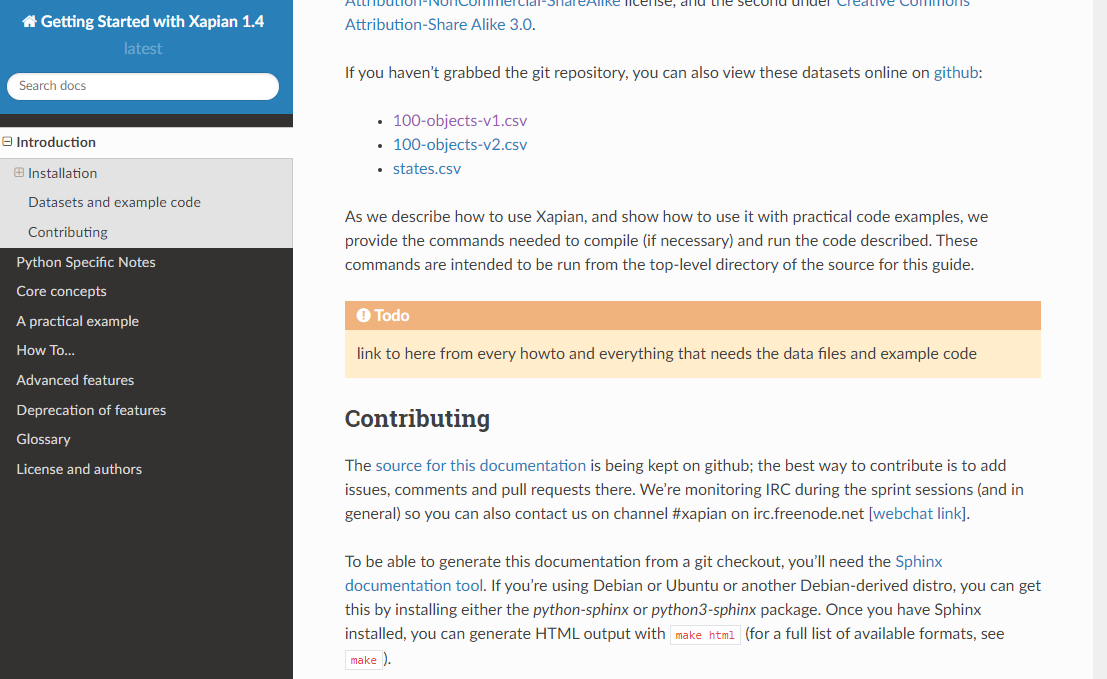
\includegraphics[width=1\linewidth]{images/xapian_doku.png}
	\caption{Screenshot von der Xapian-Dokumentation}
	\label{img:xapianDoku}
\end{figure}

\subsection{Absetzen einer Anfrage und Integration in PHP}

Xapian besitzt keine REST-Schnittstelle. Daher muss hier per Befehl direkt auf mit Systemaufrufen gearbeitet werden. Ich konnte leider nicht die Remote Ausführung testen, da der Aufwand, um die PHP-Erweiterung auf Windows zu bauen, das Zeitkontingent für den Test überschreitet. Daher habe ich die Datei direkt auf den Server ausgeführt, was bei der Laufzeit bedacht werden muss. 

Der Grund, warum eine eigene Zeile für den Buchstaben ausgewiesen werden muss, ist, dass Xapian generell nur Volltext ausweist. Ich habe zuerst versucht mit Wildcards zu arbeiten, allerdings ergab sich dabei dasselbe Problem, wie bei den anderen Suchmaschinen. Generell um in Xapian Volltext-Suche nutzen zu können, müssen gewissen Flags gesetzt werden.

\begin{lstlisting}[language=php, frame=single, label={lst:managedSchema}, 
	morekeywords={type,uninvertible,indexed,stored,field,multiValued, name}] 
// Require xapian.php and declare variables

$db = new XapianDatabase('db'); //Open Database

$queryParser = new XapianQueryParser();
//Set Prefix for Search
$queryParser->add_prefix("searchIndexLetter", "K"); 
$query = $queryParser->parse_query('S'); // Parse Query

//Loop for and time Results
// Use an Enquire object on the database to run the query
$enquire = new XapianEnquire($db);
$enquire->set_query($query);
$matches = $enquire->get_mset(0, 2147483647)->begin();
foreach ($matches as $pointer){
	$doc = $matches->get_document()->get_data();
	//$fields = json_decode($doc);
	$count++;
}
// Output Time for Run
//End Loop 
// Output Median Time
	
\end{lstlisting}

Nachdem der Query die ersten hundert Male durchlief, war die Zeit mit 0.0044 Sekunden im Durchschnitt für die 15661 Ergebnisse sehr gering. Dies liegt daran, dass die Ergebnisse erstmal nur Pointer auf die kompletten Daten sind. Um nun alle Daten zu erhalten, muss nochmals ein gesonderter Befehl geschickt werden. Deswegen ist im Code ab Zeile 15 auch eine For-Schleife, welche die Datensätze für alle Pointer holt. Foreach verschiebt dabei automatisch den Pointer von den Ergebnissen. Wichtig ist, dass der Count ein Step ist, der theoretisch die Laufzeit erhöht. Allerdings habe ich diesen hingenommen, um festzustellen, ob immer alle Ergebnisse korrekt geliefert werden. 
Die auskommentierte Zeile würde das Objekt nun als Array mit Indices zurückgeben. 

Bei den Lauf mit der Foreach-Schleife, lief der Query im Durchschnitt 0.22 Sekunden, was immernoch sehr schnell ist. Allerdings muss dabei bedacht werden, dass das die Query hierbei auf den System ausgeführt wurde und nicht, wie bei den anderen Suchmaschinen, von meinen PC an den Server gesendet wurde. 

